\documentclass{standalone}
\usepackage{../../../../preamble_tikz}

\begin{document}
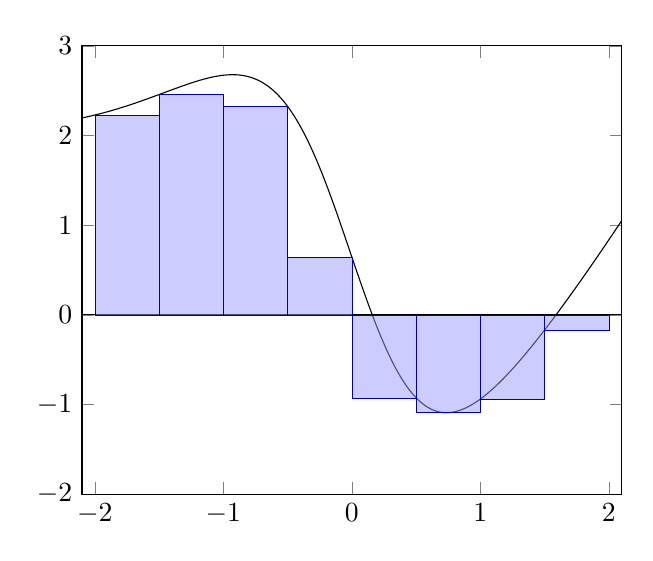
\begin{tikzpicture}[
    declare function={
        f(\x)=0.2*(0.01*(322+3*\x*(98+\x*(37+\x)))-24*\x/(1+\x*\x));
      }
  ]
  \begin{axis}[xmin=-2.1,xmax=2.1,ymin=-2,ymax=3]
    \addplot [thin,samples=200,smooth,black] {f(x)};
    \addplot [thin,samples=1,smooth,black] {0};
    \filldraw[very thin, fill=blue!40!white, draw=blue!70!black, fill opacity=0.5] (-2,0) rectangle (-2+0.5,{f(-2)});
    \filldraw[very thin, fill=blue!40!white, draw=blue!70!black, fill opacity=0.5] (-2+0.5,0) rectangle (-2+2*0.5,{f(-2+0.5)});
    \filldraw[very thin, fill=blue!40!white, draw=blue!70!black, fill opacity=0.5] (-2+2*0.5,0) rectangle (-2+3*0.5,{f(-2+3*0.5)});
    \filldraw[very thin, fill=blue!40!white, draw=blue!70!black, fill opacity=0.5] (-2+3*0.5,0) rectangle (-2+4*0.5,{f(-2+4*0.5)});
    \filldraw[very thin, fill=blue!40!white, draw=blue!70!black, fill opacity=0.5] (-2+4*0.5,0) rectangle (-2+5*0.5,{f(-2+5*0.5)});
    \filldraw[very thin, fill=blue!40!white, draw=blue!70!black, fill opacity=0.5] (-2+5*0.5,0) rectangle (-2+6*0.5,{f(0.7362)});
    \filldraw[very thin, fill=blue!40!white, draw=blue!70!black, fill opacity=0.5] (-2+6*0.5,0) rectangle (-2+7*0.5,{f(-2+6*0.5)});
    \filldraw[very thin, fill=blue!40!white, draw=blue!70!black, fill opacity=0.5] (-2+7*0.5,0) rectangle (-2+8*0.5,{f(-2+7*0.5)});
  \end{axis}
\end{tikzpicture}
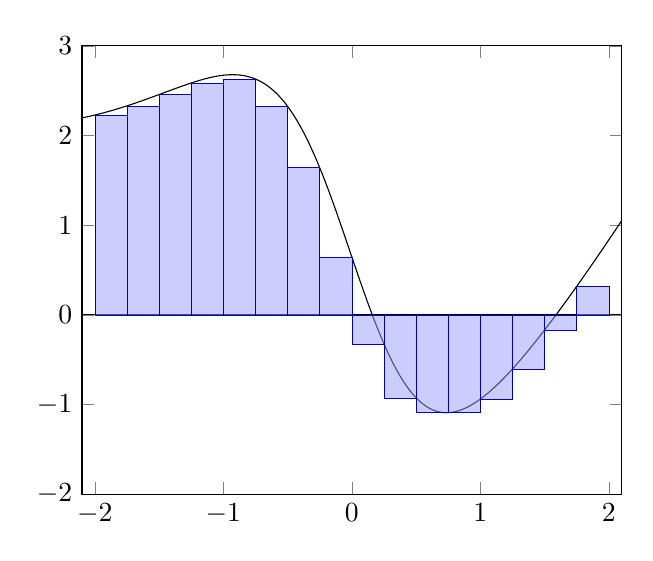
\begin{tikzpicture}[
    declare function={
        f(\x)=0.2*(0.01*(322+3*\x*(98+\x*(37+\x)))-24*\x/(1+\x*\x));
      }
  ]
  \begin{axis}[xmin=-2.1,xmax=2.1,ymin=-2,ymax=3]
    \addplot [thin,samples=200,smooth,black] {f(x)};
    \addplot [thin,samples=1,smooth,black] {0};
    \filldraw[very thin, fill=blue!40!white, draw=blue!70!black, fill opacity=0.5] (-2,0) rectangle (-2+0.25,{f(-2)});
    \filldraw[very thin, fill=blue!40!white, draw=blue!70!black, fill opacity=0.5] (-2+0.25,0) rectangle (-2+2*0.25,{f(-2+0.25)});
    \filldraw[very thin, fill=blue!40!white, draw=blue!70!black, fill opacity=0.5] (-2+2*0.25,0) rectangle (-2+3*0.25,{f(-2+2*0.25)});
    \filldraw[very thin, fill=blue!40!white, draw=blue!70!black, fill opacity=0.5] (-2+3*0.25,0) rectangle (-2+4*0.25,{f(-2+3*0.25)});
    \filldraw[very thin, fill=blue!40!white, draw=blue!70!black, fill opacity=0.5] (-2+4*0.25,0) rectangle (-2+5*0.25,{f(-2+5*0.25)});
    \filldraw[very thin, fill=blue!40!white, draw=blue!70!black, fill opacity=0.5] (-2+5*0.25,0) rectangle (-2+6*0.25,{f(-2+6*0.25)});
    \filldraw[very thin, fill=blue!40!white, draw=blue!70!black, fill opacity=0.5] (-2+6*0.25,0) rectangle (-2+7*0.25,{f(-2+7*0.25)});
    \filldraw[very thin, fill=blue!40!white, draw=blue!70!black, fill opacity=0.5] (-2+7*0.25,0) rectangle (-2+8*0.25,{f(-2+8*0.25)});
    \filldraw[very thin, fill=blue!40!white, draw=blue!70!black, fill opacity=0.5] (-2+8*0.25,0) rectangle (-2+9*0.25,{f(-2+9*0.25)});
    \filldraw[very thin, fill=blue!40!white, draw=blue!70!black, fill opacity=0.5] (-2+9*0.25,0) rectangle (-2+10*0.25,{f(-2+10*0.25)});
    \filldraw[very thin, fill=blue!40!white, draw=blue!70!black, fill opacity=0.5] (-2+10*0.25,0) rectangle (-2+11*0.25,{f(0.7362)});
    \filldraw[very thin, fill=blue!40!white, draw=blue!70!black, fill opacity=0.5] (-2+11*0.25,0) rectangle (-2+12*0.25,{f(-2+11*0.25)});
    \filldraw[very thin, fill=blue!40!white, draw=blue!70!black, fill opacity=0.5] (-2+12*0.25,0) rectangle (-2+13*0.25,{f(-2+12*0.25)});
    \filldraw[very thin, fill=blue!40!white, draw=blue!70!black, fill opacity=0.5] (-2+13*0.25,0) rectangle (-2+14*0.25,{f(-2+13*0.25)});
    \filldraw[very thin, fill=blue!40!white, draw=blue!70!black, fill opacity=0.5] (-2+14*0.25,0) rectangle (-2+15*0.25,{f(-2+14*0.25)});
    \filldraw[very thin, fill=blue!40!white, draw=blue!70!black, fill opacity=0.5] (-2+15*0.25,0) rectangle (-2+16*0.25,{f(-2+15*0.25)});
  \end{axis}
\end{tikzpicture}
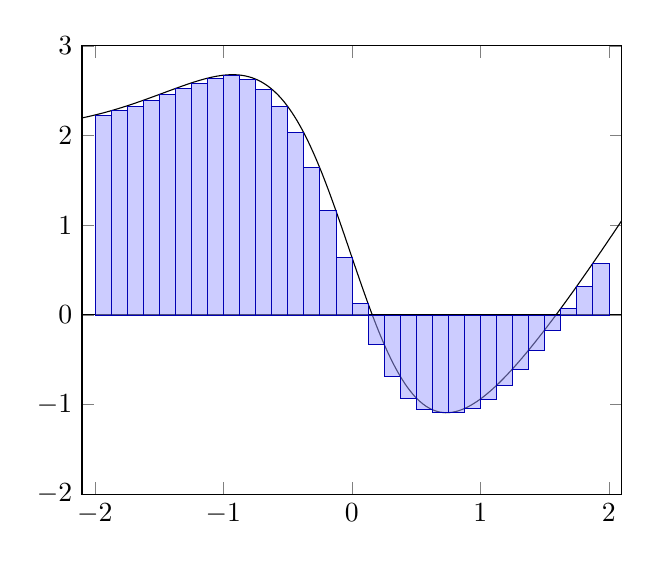
\begin{tikzpicture}[
    declare function={
        f(\x)=0.2*(0.01*(322+3*\x*(98+\x*(37+\x)))-24*\x/(1+\x*\x));
      }
  ]
  \begin{axis}[xmin=-2.1,xmax=2.1,ymin=-2,ymax=3]
    \addplot [thin,samples=200,smooth,black] {f(x)};
    \addplot [thin,samples=1,smooth,black] {0};
    \filldraw[very thin, fill=blue!40!white, draw=blue!70!black, fill opacity=0.5] (-2,0) rectangle (-2+0.125,{f(-2)});
    \filldraw[very thin, fill=blue!40!white, draw=blue!70!black, fill opacity=0.5] (-2+0.125,0) rectangle (-2+2*0.125,{f(-2+0.125)});
    \filldraw[very thin, fill=blue!40!white, draw=blue!70!black, fill opacity=0.5] (-2+2*0.125,0) rectangle (-2+3*0.125,{f(-2+2*0.125)});
    \filldraw[very thin, fill=blue!40!white, draw=blue!70!black, fill opacity=0.5] (-2+3*0.125,0) rectangle (-2+4*0.125,{f(-2+3*0.125)});
    \filldraw[very thin, fill=blue!40!white, draw=blue!70!black, fill opacity=0.5] (-2+4*0.125,0) rectangle (-2+5*0.125,{f(-2+4*0.125)});
    \filldraw[very thin, fill=blue!40!white, draw=blue!70!black, fill opacity=0.5] (-2+5*0.125,0) rectangle (-2+6*0.125,{f(-2+5*0.125)});
    \filldraw[very thin, fill=blue!40!white, draw=blue!70!black, fill opacity=0.5] (-2+6*0.125,0) rectangle (-2+7*0.125,{f(-2+6*0.125)});
    \filldraw[very thin, fill=blue!40!white, draw=blue!70!black, fill opacity=0.5] (-2+7*0.125,0) rectangle (-2+8*0.125,{f(-2+7*0.125)});
    \filldraw[very thin, fill=blue!40!white, draw=blue!70!black, fill opacity=0.5] (-2+8*0.125,0) rectangle (-2+9*0.125,{f(-2+9*0.125)});
    \filldraw[very thin, fill=blue!40!white, draw=blue!70!black, fill opacity=0.5] (-2+9*0.125,0) rectangle (-2+10*0.125,{f(-2+10*0.125)});
    \filldraw[very thin, fill=blue!40!white, draw=blue!70!black, fill opacity=0.5] (-2+10*0.125,0) rectangle (-2+11*0.125,{f(-2+11*0.125)});
    \filldraw[very thin, fill=blue!40!white, draw=blue!70!black, fill opacity=0.5] (-2+11*0.125,0) rectangle (-2+12*0.125,{f(-2+12*0.125)});
    \filldraw[very thin, fill=blue!40!white, draw=blue!70!black, fill opacity=0.5] (-2+12*0.125,0) rectangle (-2+13*0.125,{f(-2+13*0.125)});
    \filldraw[very thin, fill=blue!40!white, draw=blue!70!black, fill opacity=0.5] (-2+13*0.125,0) rectangle (-2+14*0.125,{f(-2+14*0.125)});
    \filldraw[very thin, fill=blue!40!white, draw=blue!70!black, fill opacity=0.5] (-2+14*0.125,0) rectangle (-2+15*0.125,{f(-2+15*0.125)});
    \filldraw[very thin, fill=blue!40!white, draw=blue!70!black, fill opacity=0.5] (-2+15*0.125,0) rectangle (-2+16*0.125,{f(-2+16*0.125)});
    \filldraw[very thin, fill=blue!40!white, draw=blue!70!black, fill opacity=0.5] (-2+16*0.125,0) rectangle (-2+17*0.125,{f(-2+17*0.125)});
    \filldraw[very thin, fill=blue!40!white, draw=blue!70!black, fill opacity=0.5] (-2+17*0.125,0) rectangle (-2+18*0.125,{f(-2+18*0.125)});
    \filldraw[very thin, fill=blue!40!white, draw=blue!70!black, fill opacity=0.5] (-2+18*0.125,0) rectangle (-2+19*0.125,{f(-2+19*0.125)});
    \filldraw[very thin, fill=blue!40!white, draw=blue!70!black, fill opacity=0.5] (-2+19*0.125,0) rectangle (-2+20*0.125,{f(-2+20*0.125)});
    \filldraw[very thin, fill=blue!40!white, draw=blue!70!black, fill opacity=0.5] (-2+20*0.125,0) rectangle (-2+21*0.125,{f(-2+21*0.125)});
    \filldraw[very thin, fill=blue!40!white, draw=blue!70!black, fill opacity=0.5] (-2+21*0.125,0) rectangle (-2+22*0.125,{f(0.7362)});
    \filldraw[very thin, fill=blue!40!white, draw=blue!70!black, fill opacity=0.5] (-2+22*0.125,0) rectangle (-2+23*0.125,{f(-2+22*0.125)});
    \filldraw[very thin, fill=blue!40!white, draw=blue!70!black, fill opacity=0.5] (-2+23*0.125,0) rectangle (-2+24*0.125,{f(-2+23*0.125)});
    \filldraw[very thin, fill=blue!40!white, draw=blue!70!black, fill opacity=0.5] (-2+24*0.125,0) rectangle (-2+25*0.125,{f(-2+24*0.125)});
    \filldraw[very thin, fill=blue!40!white, draw=blue!70!black, fill opacity=0.5] (-2+25*0.125,0) rectangle (-2+26*0.125,{f(-2+25*0.125)});
    \filldraw[very thin, fill=blue!40!white, draw=blue!70!black, fill opacity=0.5] (-2+26*0.125,0) rectangle (-2+27*0.125,{f(-2+26*0.125)});
    \filldraw[very thin, fill=blue!40!white, draw=blue!70!black, fill opacity=0.5] (-2+27*0.125,0) rectangle (-2+28*0.125,{f(-2+27*0.125)});
    \filldraw[very thin, fill=blue!40!white, draw=blue!70!black, fill opacity=0.5] (-2+28*0.125,0) rectangle (-2+29*0.125,{f(-2+28*0.125)});
    \filldraw[very thin, fill=blue!40!white, draw=blue!70!black, fill opacity=0.5] (-2+29*0.125,0) rectangle (-2+30*0.125,{f(-2+29*0.125)});
    \filldraw[very thin, fill=blue!40!white, draw=blue!70!black, fill opacity=0.5] (-2+30*0.125,0) rectangle (-2+31*0.125,{f(-2+30*0.125)});
    \filldraw[very thin, fill=blue!40!white, draw=blue!70!black, fill opacity=0.5] (-2+31*0.125,0) rectangle (-2+32*0.125,{f(-2+31*0.125)});
  \end{axis}
\end{tikzpicture}
\end{document}